\documentclass[5pt,openright,final]{unsa}
\title{Base de datos basado en grafos de investigadores de Concytec para un análisis de diversas perspectivas}
\author{Rodrigo Alexander Mamani Sucacahua}%
% of being the case
\date{10 de octubre del 2021}
\dedicate{A Dios, por todo lo que me ha dado, a todos los profesores
por sus enseñanzas. a amigos y familiares por el apoyo.}


\usepackage[options ]{algorithm2e}
\usepackage[table,xcdraw]{xcolor}
\usepackage{glossaries}


\setcounter{secnumdepth}{3}
\begin{document}%%%%%%%%-------------------------------------------------------
% Keywords command
\providecommand{\keywords}[1]
{
  \small	
  \textbf{\textit{Keywords---}} #1
}
    \makeSecondCover %
\begin{frontmatter}

%\approved{\cuatro}%  {\tres} or {\cuatro}

%\dedicatory
%\begin{singlespace}
%\tableofcontents \listoffigures \listoftables \pagebreak
%\end{singlespace}
%\myAcknowledgements{Agradecimientos}%
%\myResumen{Resumen}%
%\myAbstrac{Abstract}%
\end{frontmatter}%
\pagestyle{fancyplain}
\chapter{Introducción General}

\section{Introducción}
Las universidades públicas y privadas presentan la necesidad de contactar,contratar y encontrar investigadores en áreas en específico, ya sea para ayudar a los alumnos en su asesoramiento para sus proyectos de tesis o para dirigir proyectos de pregrado, para estos fines se evaluan de diversas maneras y puntos de referencia dados por los interesados. Esta toma de decisiones ayuda a los interesados tener veracidad y respaldo de calidad en el área de investigación.Para esto se opta a buscar en bases de datos públicas las cuales brindan dicha información realizando largas búsquedas para encontrar a los investigadores de su interés. Concretamente en el Perú la página de DINA de Concytec brinda información de los investigadores como bibliografía, experiencia profesional, datos académicos, producción científicas, proyectos de investigación entre otros dotas los cuales pueden ser de gran utilidad para dicho objetivo .

\section{Definición del problema}
Las búsquedas largas en páginas como DINA son muy engorrosas ya que no solo es encontrar a un sector de investigadores de su interés sino también leer los datos en forma de texto y sus curriculum vitae respectivos.
Además, existen datos abstractos del interés académico que no se muestran en dicha página las cuales las relaciones de estas a menudo son hasta necesario consultar con el mismo investigador para saber si tiene lo que se busca o no, como que si tiene contacto con el extrangero, si conoce a colegas o investigadores de su rama entre otras cosas.\\
%%%%%%Así como ya esta, ¿que problema existe actualmente?, respecto a lo
%que quieres proponer o mostrar.
Al plantear el traslado de los datos a una base de datos lo mas común es hacerlo a una base de datos relacional en lenguaje SQL , sin embargo, al momento de hacer consultas para encontrar un dato determinado se usan demasiados comandos de consultas JOIN , los cuales, si bien es cierto que es mas fácil la interacción con datos existen bases de datos que pueden brindar los datos requeridos de manera óptima como una base de datos basada en grafos.
%\section{Justificación}

%¿porque estas desarrollando esta tesis?

\section{Objetivos}
\subsection{Objetivo General}
\begin{itemize}
    \item Analizar el funcionamiento de la base de datos basada en grafos de DINA.
\end{itemize}

\subsection{Objetivos Específicos}
\begin{itemize}
\item  Realizar el traslado de datos de la página de DINA a una base de datos basada en gráfos
\item Usar Neo4j para probar el funcionamiento con datos de investigadores de la UNSA
\item Realizar un análisis de algunas relaciones hechas en cypher (lenguaje de consultas de Neo4j)
\item Mostrar gráfos de las consultas obtenidas.
\end{itemize}
\section{Hipótesis}
La herramienta Neo4j es muy útil para la creación y el análisis base de datos.
\section{Estado del Arte}
El enfoque dado para el muestreo de investigadores es eficiente para la búsqueda concreta de los investigadores de interés y se demuestra el funcionamiento de esta base de datos basa den grafos y cuan eficiente es este modelo \cite{afandi2020university}.
Dina no es la única fuente de datos de investigadores a nivel mundial, en este artículo plantea la visualización de datos de DSPACE en Neo4j y Dephi herramientas de visualización de código de acceso libre y apliaciones desktop \cite{aryani2017visualising}.
Para tener un buen análisis de una herramienta de creación de base de datos basado en grafos como Neo4j se debe evaluar como el back-end trabajado en esta aplicaciónayuda a los desarrolladores para su fácil entendimiento\cite{holzschuher2013performance}.\\
Para analizar a fondo la creación de la base de datos se deben evaluar la relación entre atributos y la asociación que estos presentan con la base de datos.\cite{lu2017analysis}.También se deben evaluar las consultas y transacciones que se pueden realizar en la base de datos creada en Neo4j\cite{vukotic2015neo4j}.\\
Neo4j al ser una herramienta basada en grafos, es evidente que la base de datos creada sea basada en grafos, esta puede ser planteada en una base de datos distribuida como las social networks la cual ,tal como la base de datos general, de Neo4j esta también puede ser visualizada de manera óptima\cite{agudo2020base}.\\
Como toda aplicación Neo4j tiene ventajas y desventajas en su uso, las cuales mediante comparaciones con diversas aplicaciones pueden ayudar al usuario a decidir si es factible o no usar dicha herramienta\cite{fernandes2018graph}.Las limitaciones que esta herramienta presenta pueden ser evaluados por su interacción de la base de datos con las consultas y con los datos los cuales demuestran que Neo4j es una herramienta optimizable\cite{miller2013graph}.\\
El análisis de una herramienta como Neo4j también puede ser evaluado por el tiempo de demora de la creación de la base de datos y su complejidad de consultas comparadas con otra herramienta como PostgreSQL.\cite{stothers2020can}.
Neo4j no solo sirve para bases de datos convensionales , sino también ayudan para el mejor control de la semántica e interacción de las bases de datos como las redes sociales y web semántica\cite{guia2017graph}.

\section{Marco Teórico}

\section{Variables de investigación}
\subsection{Variables Independientes}
\begin{itemize}
    \item Análisis
    \item Perspectivas
\end{itemize}
\subsection{Variables Dependientes}
\begin{itemize}
    \item Base de datos basado en grafos
    \item Investigadores de Concytec
\end{itemize}
%\section{Organización de la tesis}

%Una breve descripción de cada uno de los capítulos que estas desarrollando desde el CAP 2 hasta el capitulo antes del apéndice.

\chapter{Técnicas a reproducir}
\hrule  \vspace*{0.5cm}
%\section{Bases teóricas}
\section{Base de datos basado en Neo4j}
\subsection{Abstract}
Con el desarrollo de Internet, el crecimiento de los datos cinematográficos
rápidamente, la relación entre los datos de la película se vuelve más y
más complicado. Las relaciones entre películas, actores
y los escritores son información importante tanto para los productores de cine
y audiencias. El sitio web de datos de películas no solo necesita almacenar
vídeos de películas, también necesitan almacenar información sobre
directores, escritores, actores, etc.
Si tales datos se almacenan en una base de datos relacional, el
las conexiones entre diferentes tablas se pueden establecer a través de
llave. Sin embargo, cuando hay muchas relaciones, la base de datos relacional tradicional no solo tiene una gran cantidad de
redundancia de datos, pero también se vuelve difícil de actualizar
dinamicamente. Además, es difícil realizar consultas complejas
relaciones entre dos entidades. Por ejemplo, cuando
quieren saber si los principales productores de las dos películas
tienes una coproducción de otras películas, necesitas encontrar otras
películas producidas por los principales productores de las dos películas, y
luego analice si existe una intersección entre ellos.
Por lo tanto, la base de datos no relacional es una buena elección para
investigar y procesar datos de películas. Neo4j, que es un
excelente herramienta de base de datos de gráficos, almacena datos en forma de gráfico que puede representar objetos con nodos, aristas y propiedades \cite{lu2017analysis}.
En consecuencia, es adecuado para almacenar complejos y dinámicos
relaciones entre objetos de datos fílmicos, por lo que se desarrollará la recreación de la base de datos no relacional basada en grafos de Neo4j de DataFilm y su respectivo análisis.
\subsection{Neo4j}
Al momento de usar o crear bases de datos, las bases de datos relacionales han sido dominantes durante mucho tiempo.
Con la aplicación de Wed 2.0, el auge de las redes sociales, la dependencia y la complejidad de los datos internos aumentan gradualmente,
Cada vez surgen más problemas en las bases de datos relacionales. Luego,
apareció la base de datos basado en grafos.\\
En los últimos años ha habido una enorme cantidad de bases de datos basado en grafos de alto rendimient, existen multiples herramientas que trabajan con el diseño y la arquitectura de dicha base de datos entre ellas tenemos a Neo4j.
Esta herramienta en específico trabaja en la corriente principal de un software de código abierto basado en Jav, actualmente su kernel es un motor de gráficos muy rápido, con la recuperación de datos, con dos fases del envío, soporte para transacciones XA y otras características del producto de base de datos.
Neo4j es una base de datos orientada a la red, es decir, una base de datos integrada con motor de persistencia Java totalmente transaccional basado en disco que almacena datos estructurados en redes en lugar de tablas.
El lenguaje de esta herramienta es llamado Cypher el cual presenta sus propios comandos y formas de crear una base de datos con sus respectivos atributos.
En este modelo, los datos de dominio se expresan en un "espacio de nodos" la cual esta compuesta de: una red de nodos, relaciones y propiedades (pares clave-valor), en comparación con las tablas del modelo relacional, que trabajan con filas y columnas. Las relaciones son objetos de primera clase y pueden
también se tener  propiedades, revelando el contexto de cuales son los nodos con los que se interactúan. 
\subsection{Creación de la base de datos}
Para crear una base de datos basada en grafos debemos saber el funcionamiento de este y como empezar a crearla.La asociación es similar al borde en un grafo dirigido,El borde de esta base de datos consta de tres elementos: el nodo inicial, el nodo final y el tipo.
La orientación del borde aclara aún más la semántica y la
relación entre nodos.En la Figura \ref{fig:borde} vemos que los atributos de los nodos y las relaciones se pueden definir por clave-valor. Actores, directores,
escritores y películas son entidades diferentes cuando los datos de la película son almacenados, la base de datos de Neo4j no solo necesita almacenar entidades, sino también necesita almacenar las relaciones entre entidades.
\begin{figure}[H]
    \centering
    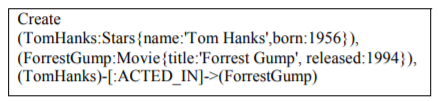
\includegraphics[scale=0.8]{Graficos/ejemplo.png}
    \caption{Ejemplo de la creación de un borde  \cite{lu2017analysis}.}
    \label{fig:borde}
\end{figure}
\subsection{Consultas y resultados}
En la Figura \ref{fig:grafo_bd} vemos el grafo de la película <The Green Mill> como el punto de partida, se crea una pequeña base de datos con 19 nodos y 19
relaciones como se muestra en la siguiente figura. En la figura tambien veremos que, el nodo de color verde significa que es un nodo de película,el amarillo significa que la etiqueta pertenece al nodo del actor,la etiqueta rosa significa que es un escritor, etiqueta azul significa que es un director, se utilizan diferentes colores para representar diferentes etiquetas y por ende diferentes tipos de nodos a construir.

\begin{figure}[H]
    \centering
    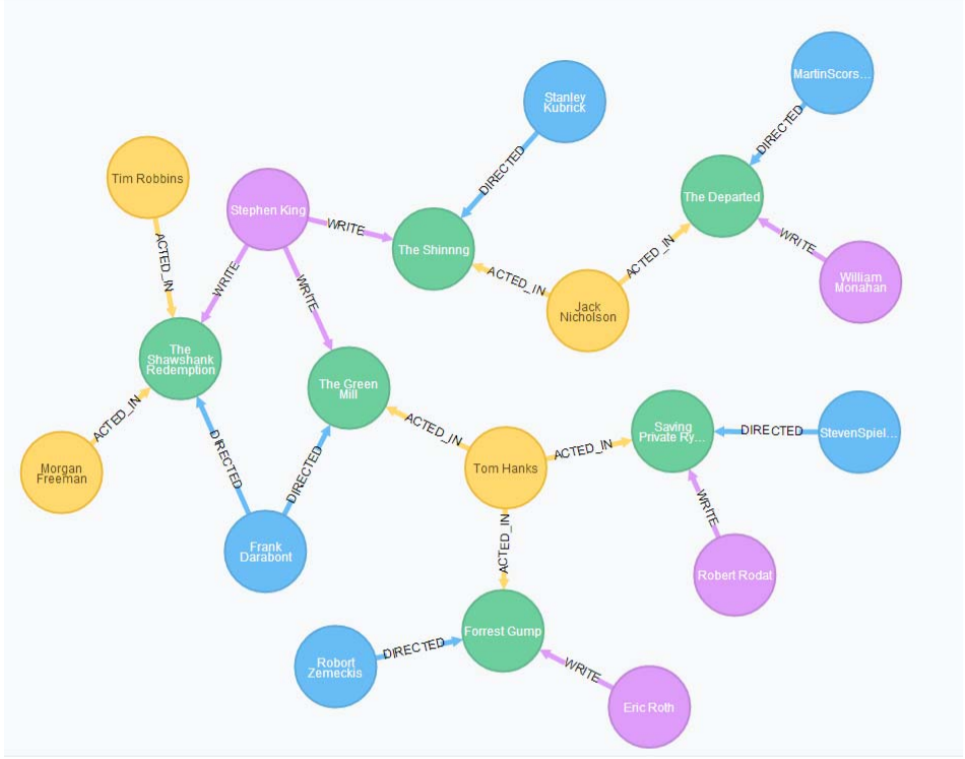
\includegraphics[scale=0.5]{Graficos/bd.png}
    \caption{Base de datos de películas en formato grafo \cite{lu2017analysis}.}
    \label{fig:grafo_bd}
\end{figure}
\newpage
Aquí hay un ejemplo,en la Figura \ref{fig:consulta} según el usuario ha visto la película.
<La redención Shawshank> y <Forrest Gump>, el sistema recomienda otras películas que se relacionen con las dos películas al usuario.
Por análisis encontramos que Tom Hanks actuó en <Forrest Gump>
y <The Green Mill>, el director Frank Darabont no solo
dirigió <THE Green Mill> pero también dirigió <The Shawshank
Redención>, por lo que encontramos la relación potencial entre la
película <Forrest Gump>, <The Shawshank Redemption> y
<The Green Mill>, por lo que podemos recomendar la película <The
Green Mill> al usuario. La siguiente es la consulta en el lenguaje Cypher muestra la consulta para este ejemplo.
\begin{figure}[H]
    \centering
    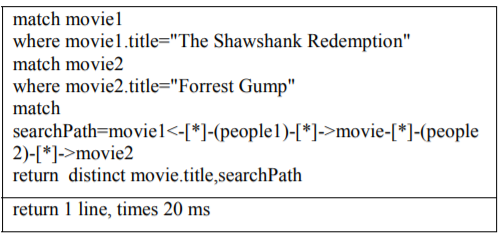
\includegraphics[scale=0.8]{Graficos/cypher1.png}
    \caption{Consulta en lenguaje Cypher \cite{lu2017analysis}.}
    \label{fig:consulta}
\end{figure}
Ya que la herramienta Neo4j nos brinda la opción de representar nuestra base de datos en una arquitectura de grafos usaremos esta opción para una mejor interpretación y después veremos el gráfico de dicha consulta en la Figura \ref{fig:rep} y como esta representado sus relaciones y nodos correspondientes.
\begin{figure}[H]
    \centering
    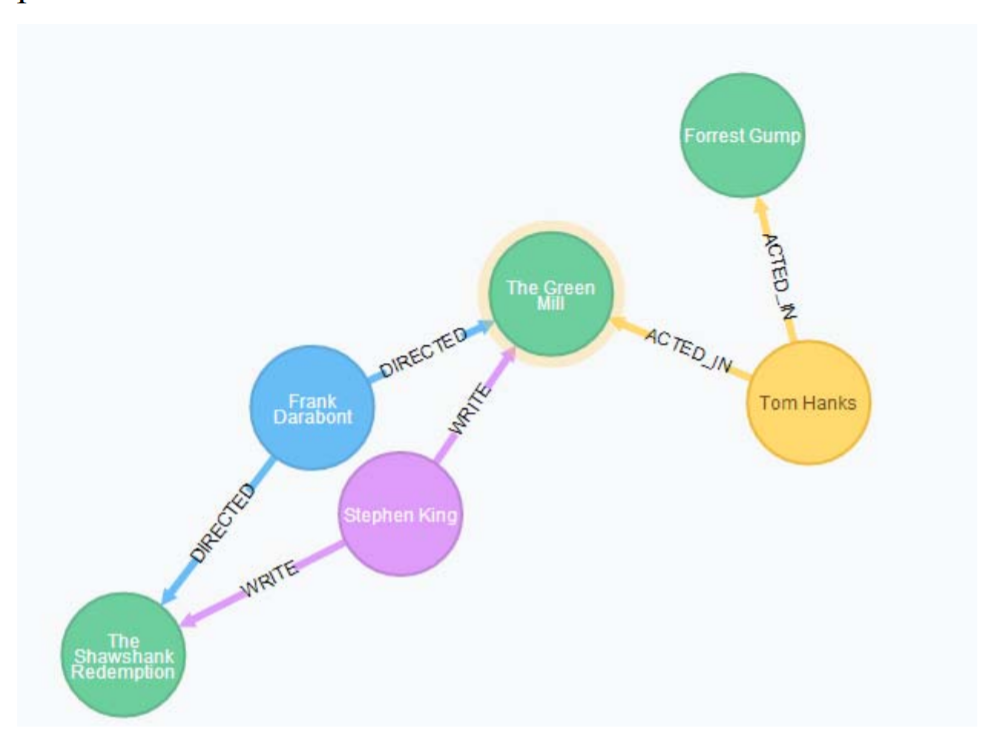
\includegraphics[scale=0.5]{Graficos/consultagraph.png}
    \caption{Representación en grafos de la consulta anterior \cite{lu2017analysis}.}
    \label{fig:rep}
\end{figure}
\section{Base de datos de investigación universitaria en Neo4j}
\subsection{Abstract}
En su mayoría, los datos relacionados con la investigación se modelan
usando una base de datos relacional optimizada para el proceso de transacciones, esto se debe a que es el tipo de base de datos mas común para dicho trabajo. En muchos casos, esta solución es eficaz y eficiente, lo suficiente como para responder consultas básicas e transacciones sencillas. Sin embargo, cuando los usuarios solicitan un análisis más detallado, más expansivo, con múltiples perspectivas y, a veces, un mayor análisis abstracto, la base de datos relacional lucha por proporcionar respuestas. Este estudio propone una base de datos basado en grafos de investigación implementado usando neo4j como la herramienta de creación para responder a los problemas.La base de datos permite que la
universidad pueda analizar el trabajo individual y colaborativo de los investigadores en conjunto de compañeros investigadores dentro y fuera de las
universidades. El estudio concluye que el gráfico de investigación que muestra que la implementación de la base de datos es más eficiente para responder
preguntas que la implementación de la base de datos relacional.
\subsection{Métodología}
Para la recolección de datos para la creación de nuestra base de datos basada en grafos se optó por evaluar las multiples fuentes de información consistentes y de buena procedencia que se pueden encontrar en la nube.
Entre aquellas podemos encontrar a Google Scholar.\\
Google Scholar es una plataforma denominado SINTA (Índice de Ciencia y Tecnología). Ristekbrin
(Ministerio de Investigación y Tecnología / Investigación Nacional y
Innovation Body) de Indonesia actualmente alberga SINTA.
SINTA utiliza datos de Google Scholar y otros
fuentes y luego calcula las capacidades de los investigadores,
instituciones y revistas en Indonesia. Los resultados son entonces
puesto a disposición del público de forma gratuita. Google Scholar
presenta ventajas que vale la pena destacar com los hechos que Google
Scholar ofrece referencias académicas más actualizadas. Existen
también API (interfaces de programación de aplicaciones) en varios
plataformas de programación creadas por desarrolladores que los investigadores,
profesionales y el público en general pueden utilizar para conectarse a
Google Scholar y recuperar datos de él de forma gratuita para académicos
con fines de investigación.
\subsection{Resultados}
Primeramente mostramos la creación de nuestra base de datos basada en grafos y usando como fuente de información la plataforma de google scholar.
La base de datos de grafos resultante de este estudio de caso consiste
de 12 etiquetas de nodo, 15 relaciones y 33 claves de propiedad.
La Tabla \ref{fig:tab_1} muestra todos los nombres de las etiquetas de los nodos, y la Tabla \ref{fig:tab_2} muestra los relación entre nodos.
\begin{figure}[H]
    \centering
    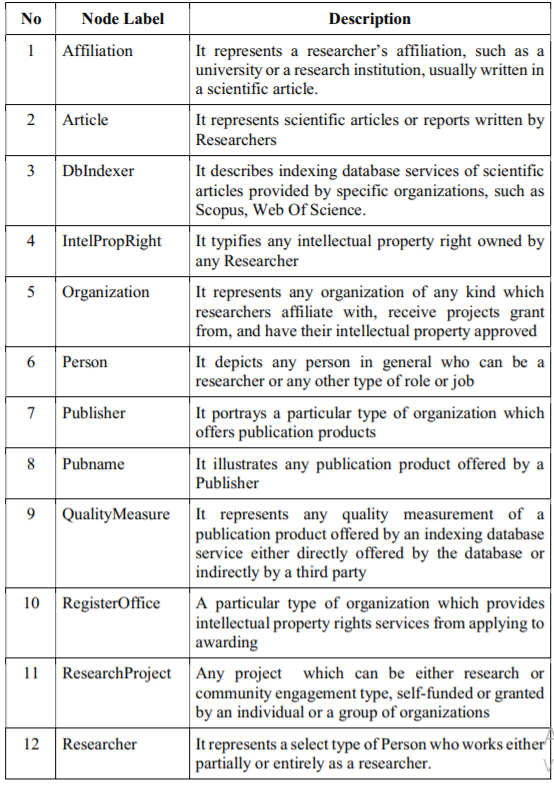
\includegraphics[scale=0.7]{Graficos/nodos.png}
    \caption{Nodos de la base de datos de investigación \cite{afandi2020university}.}
    \label{fig:tab_1}
\end{figure}
\begin{figure}[H]
    \centering
    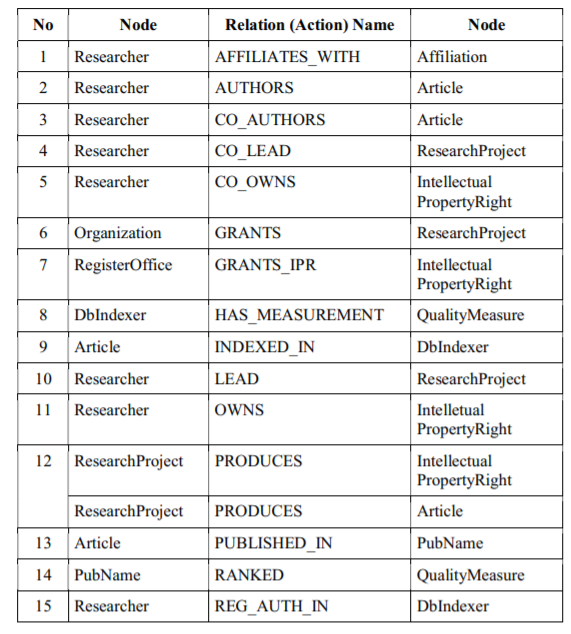
\includegraphics[scale=0.7]{Graficos/relaciones.png}
    \caption{Relaciones basado en los nodos de la base de datos de investigación \cite{afandi2020university}.}
    \label{fig:tab_2}
\end{figure}
La consulta de grafos escrita en Cypher como se muestra en la Figura \ref{fig:cypher}  es eficiente y simple. Podría decirse que puede ser formulado y realizado por trabajadores del conocimiento con menos experiencia que recibieron la formación previa y equipado con información tal como nodo y relación de nodo.
Además, la información visual que se muestra también es informativa.
y adecuado para diferentes niveles de espectadores, desde el conocimiento
trabajadores a ejecutivos.
 Una consulta más larga para responder a la misma pregunta en un relacional
es simulada en la Figura \ref{fig:sql}. La diferencia es clara. En
una base de datos relacional, el requisito debe ser muy explícito
por adelantado para que se traduzca correcta y cuidadosamente en consultas
antes de decidir qué tablas unir en qué columnas y
qué campos deben recuperarse. De hecho, requiere algunos
nivel de experiencia técnica para ejecutarlo.
\begin{figure}[H]
    \centering
    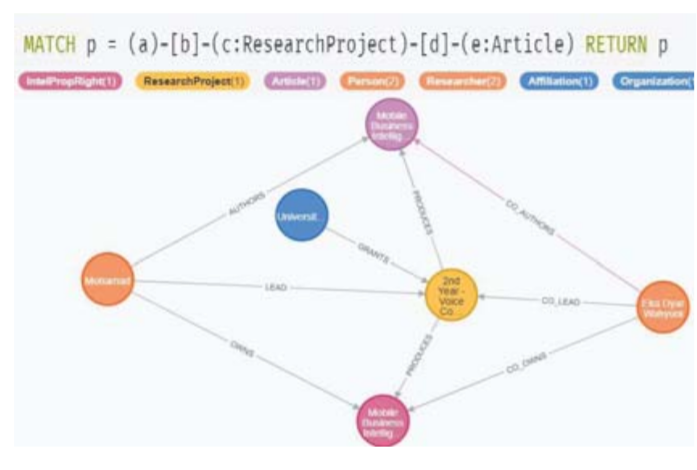
\includegraphics[scale=0.6]{Graficos/caso1.png}
    \caption{Consulta en lenguaje Cypher para la base de datos basada en grafos \cite{afandi2020university}.}
    \label{fig:cypher}
\end{figure}
\begin{figure}[H]
    \centering
    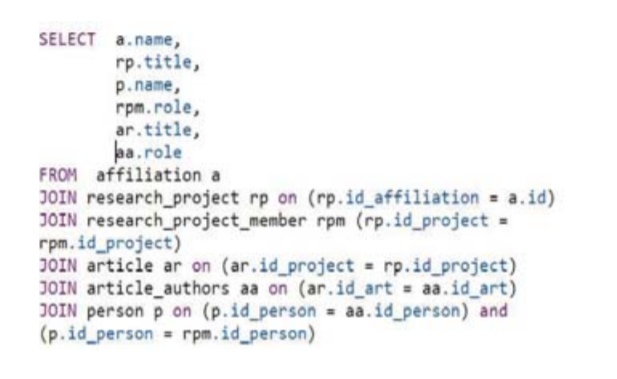
\includegraphics[scale=0.7]{Graficos/caso1_1.png}
    \caption{Consulta en SQL para la base de datos relacional \cite{afandi2020university}.}
    \label{fig:sql}
\end{figure}
\chapter{Marco teórico}
\hrule  \vspace*{0.5cm}
\section{Antecedentes}
%evidencias 
%tesis referentes al tema
\subsection{Bases de datos}
Un aspecto clave del diseño de una base de datos es asegurar que el
La base de datos contiene solo valores de datos válidos consistentes con
semántica de la base de datos incluso en presencia de:
\begin{itemize}
    \item Inserciones
    \item Eliminaciones
    \item Actualizaciones
\end{itemize}
Las restricciones simplifican las aplicaciones del sistema de base de datos
realizar comprobaciones para garantizar la validez de los datos y
consistencia.\\
Esta verificación centralizada también es más confiable ya que la aplicación puede no realizar una o más de las comprobaciones.

Una base de datos solo debe contener datos válidos y consistentes
en todo momento con la posible excepción en medio de
actualizaciones \cite{gehani1990introduction}.
Algunos tipos de validez de datos se pueden garantizar mediante SQL
limitaciones.
Ejemplos:
\begin{itemize}
    \item Los estados se identifican utilizando sus abreviaturas de dos letras.
    \item Los valores deben estar dentro de un rango específico.
    \item Los campos de datos son obligatorios y no se pueden omitir.
    \item Los valores de una columna deben ser únicos.
\end{itemize}
Ejemplos de restricciones complejas de bases de datos:
\begin{itemize}
    \item Las abreviaturas de estado de 2 letras representan abreviaturas de estado válidas.
    \item Los códigos postales representan códigos postales válidos y coinciden con las direcciones especificadas.
\end{itemize}
\subsection{Introducción a Base de datos basada en grafos}
Un gráfico es una estructura de datos compuesta por aristas y vértices. La tecnología de base de datos de gráficos es una herramienta eficaz para modelar
datos cuando un enfoque en la relación entre entidades es una fuerza impulsora en el diseño de un modelo de datos.El Modelado de objetos y las relaciones entre ellos significan que casi cualquier cosa se puede representar en un gráfico correspondienteen un gráfico común.
El tipo admitido por la mayoría de los sistemas es el gráfico de propiedades. Los gráficos de propiedades son gráficos múltiples atribuidos, etiquetados y dirigidos \cite{miller2013graph}.

\vfill
\textbf{Ejemplo de BD basada en grafos}
\vfill

\begin{figure}[H]
    \centering
    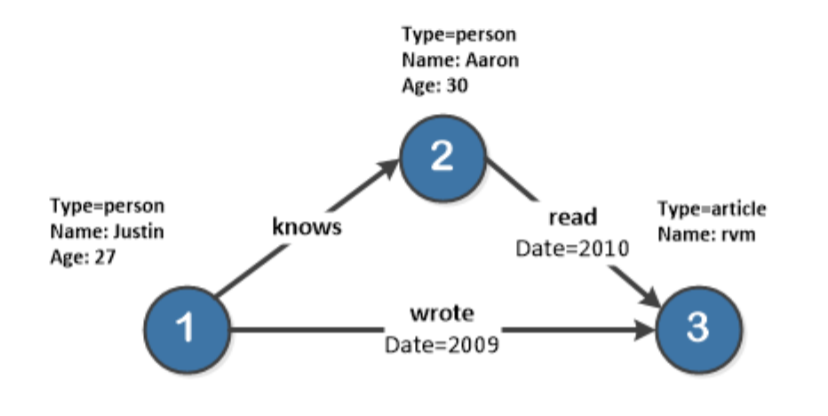
\includegraphics[scale=0.7]{Graficos/ejempbd.png}
    \caption{Ejemplo de gráfico de BDBG  Fuente: \cite{miller2013graph}.}
    \label{fig:my_label}
\end{figure}
A pesar de las limitaciones involucradas en el uso de un esquema, existen muchos beneficios, algunos de los cuales superan las restricciones implícitas en
el RDBMS. Estas bases de datos están bien respaldadas por sus respectivos proveedores, están probadas en batalla y sus las fortalezas / limitaciones son bien conocidas, tienen un lenguaje de consulta común (SQL), hay una amplia reserva de talentos de capacitados profesionales a los que recurrir, y estas plataformas están muy bien documentadas. Por el contrario, las bases de datos de gráficos se enfrentan a una conjunto de desafíos inherentes a su diseño.
\begin{figure}[H]
    \centering
    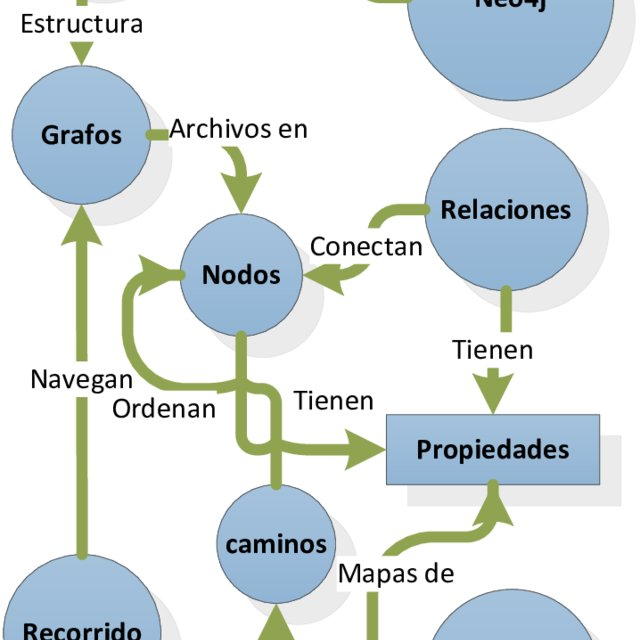
\includegraphics[scale=1]{Graficos/dbgrafo.jpg}
    \caption{Ejemplo de arquitectura de una BD basada en grafos. }
    \label{fig:my_label}
\end{figure}
\subsection{Aplicación de base de datos basado en grafos}
Las bases de datos gráficas realmente brillan cuando se trabaja en áreas donde la información sobre la interconectividad o la topología de datos es importante.
En tales aplicaciones, las relaciones entre los datos y los datos en sí suelen estar al mismo nivel . Muchas empresas tienen
desarrolló implementaciones internas para hacer frente a la necesidad de sistemas de bases de datos de gráficos\cite{miller2013graph}.\\
Ejemplos serían:
\begin{itemize}
    \item Open Graph de Facebook.
    \item Knowledge Graph de Google.
    \item FlockDB de Twitter.
\end{itemize}

\subsection{Introducción a Neo4j}
Aunque los gráficos se utilizan ampliamente durante el proceso de desarrollo de software, los desarrolladores tienden a olvidarse de los gráficos cuando se trata de la persistencia de datos. Intentamos ajustar los datos en tablas y columnas relacionales, y para normalizar y renormalizar
su estructura hasta que se vea completamente diferente de lo que está tratando de representar.
Una lista de control de acceso es un ejemplo. Este es un problema resuelto una y otra vez nuevamente en muchas aplicaciones empresariales. Por lo general, tendría tablas para usuarios, roles y recursos. Luego, tendría tablas de muchos a muchos para asignar usuarios a roles y roles a los recursos. Al final, tendrías al menos cinco tablas relacionales para representar un estructura de datos simple, que en realidad es un gráfico. Entonces usarías un objeto relacional herramienta de mapeo (ORM) para mapear estos datos a su modelo de objeto, que también es un gráfico.\\
¿No sería bueno si pudiera representar los datos en su forma natural, haciendo
mapeos más intuitivos y omitiendo el proceso repetido de "traducir" los datos
hacia y desde un motor de almacenamiento?.\\
Gracias a las bases de datos de gráficos, puede hacerlo. Bases de datos de gráficos utilizar el modelo de gráfico para almacenar datos como un gráfico, con una estructura que consta de vértices y bordes, las dos entidades utilizadas para modelar cualquier gráfico.
Además, puede utilizar todos los algoritmos de la larga historia de la teoría de grafos para resolver problemas de gráficos de manera más eficiente y en menos tiempo que usando consultas de bases de datos relacionales. \cite{vukotic2015neo4j}. 
\subsection{Graficar datos en Neo4j}
Neo4j almacena datos como vértices y bordes o, en terminología de Neo4j, nodos y relaciones. Los usuarios se representarán como nodos y las amistades se representarán como relaciones entre los nodos de usuarios. Si echa otro vistazo a la red social en la Figura \ref{fig:tiempos}, verá que no representa más que un gráfico, con los usuarios como nodos y las friendship como relaciones.
Existe una diferencia clave entre las bases de datos relacionales y Neo4j, que
se encuentran de inmediato: consulta de datos. No hay tablas ni columnas en Neo4j, tampoco hay comandos de selección y combinación basados en SQL. Entonces, ¿cómo se consulta un base de datos de gráficos?
Todos los gráficos de bases de datos, toma un poderoso concepto matemático que denota que la respuesta no es escribir una función MapReduce distribuida. Neo4j, lo muestra como teoría de grafos y lo usa como un motor poderoso y eficiente para consultar datos. Este concepto es el gráfico transversal y es una de las herramientas principales que hace que Neo4j sea tan poderoso para tratar con gráfico de datos \cite{vukotic2015neo4j}.
\begin{figure}[H]
    \centering
    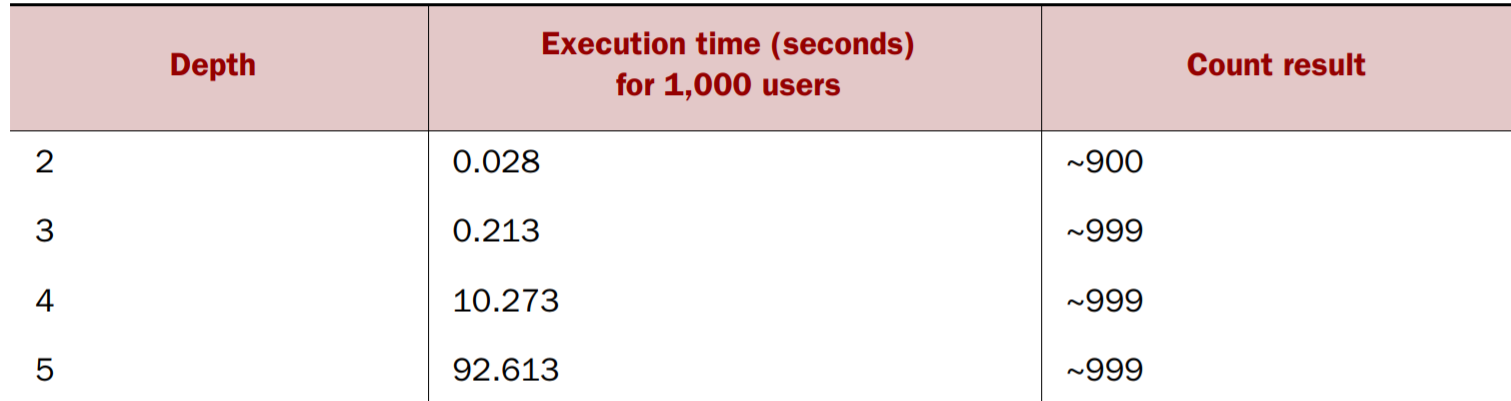
\includegraphics[scale=0.4]{Graficos/ppp.png}
    \caption{Tiempos de ejecución para múltiples consultas de combinación usando un motor de base de datos MySQL en un conjunto de datos de 1.000 usuarios}
    \label{fig:tiempos}
\end{figure}
\subsection{Neo4j en el espacio NoSQL}
Desde el comienzo del software de computadora y los datos que las aplicaciones han tenido que tratar con ha crecido enormemente en complejidad. La complejidad de los datos incluye no sólo su tamaño, también su interconexión, su estructura en constante cambio y el acceso concurrente a los datos.
Con todos estos aspectos del cambio de datos, se ha reconocido que las bases de datos relacionales, que durante mucho tiempo han sido el estándar de facto para el almacenamiento de datos, no son las más adecuadas para todos los problemas que requieren los datos cada vez más complejos. Como resultado, se ha creado una serie de nuevas tecnologías de almacenamiento, con el objetivo común de resolver
los problemas en los que las bases de datos relacionales no son buenas. Todas estas nuevas tecnologías de almacenamiento caen bajo el término general NoSQL.\\
Aunque el nombre NoSQL se atascó, no refleja con precisión la naturaleza
del movimiento, dando la impresión (errónea) de que va en contra de SQL como concepto. Un mejor nombre probablemente sería el de bases de datos no relacionales, ya que el relacional y paradigma no relacional fue el tema de discusión, mientras que SQL es sólo un lenguaje utilizado con tecnologías relacionales.
El movimiento NoSQL nació como un reconocimiento de que las nuevas tecnologías necesitaban para hacer frente a los cambios de datos. Neo4j, y las bases de datos de grafos en general, son parte del movimiento NoSQL, junto con una gran cantidad de almacenamiento más o menos relacionado con las tecnologías.
Con los rápidos desarrollos en el espacio NoSQL, su creciente popularidad y la enorme cantidad de diferentes soluciones y tecnologías para elegir, cualquiera que sea nuevo en el mundo NoSQL enfrenta muchas opciones al seleccionar la tecnología adecuada \cite{vukotic2015neo4j}. 
\subsection{Neo4j: la base de datos compatible con ACID}
La gestión de transacciones ha sido un tema de conversación destacado en las discusiones sobre las tecnologías NoSQL desde que comenzaron a ganar popularidad. Negociar atributos transaccionales para un mayor rendimiento y escalabilidad ha sido un enfoque común en tecnologías no relacionales que apuntan a big data. Algunos (como BigTable, Cassandra y CouchDB) optó por compensar la coherencia, permitiendo a los clientes leer datos obsoletos en algunos casos en un sistema distribuido (consistencia eventual). En las tiendas de valores-clave que se concentraban en el rendimiento de lectura (como Memcached), la durabilidad de los datos no generaba mucho interés. Del mismo modo, la atomicidad a nivel de una sola operación, sin la posibilidad de
envolver múltiples operaciones de bases de datos dentro de una sola transacción, es típico de las bases de datos orientadas a documentos.
Si bien cada uno de los enfoques mencionados aquí son válidos en casos de uso específicos (como el almacenamiento en caché, altos volúmenes de lectura de datos, alta carga y simultaneidad), la falta de manejo de transacciones basado en ACID suele ser el primer obstáculo cuando se trata de introducir bases de datos no relacionales a cualquier empresa o entorno corporativo. Aunque ellos
fueron ideados hace mucho tiempo para bases de datos relacionales, los atributos de transacción aún se reproducen una parte importante y fundamental en muchos casos prácticos de uso. Por tanto, Neo4j ha adoptado un enfoque diferente \cite{vukotic2015neo4j}.

\chapter{Experimentación }
\section{Técnica 1:Base de datos basado en Neo4j}
\subsection{Creación de la Base de datos}
Creamos los scripts de inicialización de la base de datos de películas.
Para esto en la Figura \ref{fig:info} vemos las característicasa de nuestra base de datos, desde los tipos de nodos y las relaciones hasta las propiedades que tienen cada nodo.
\begin{figure}[H]
    \centering
    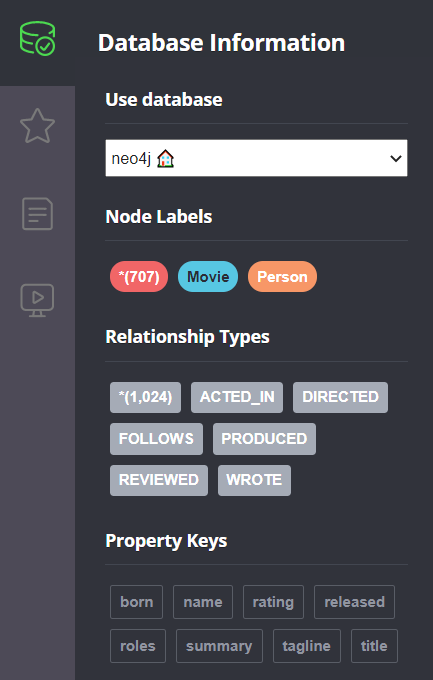
\includegraphics[scale=0.45]{Graficos/info.png}
    \caption{Datos generales de la base de datos de películas}
    \label{fig:info}
\end{figure}
A continuación en la Figura \ref{fig:graph_1} muestra el grafo del pequeño segmento tomado para la muestra de nodo y relaciones correspondientes.
\begin{figure}[H]
    \centering
    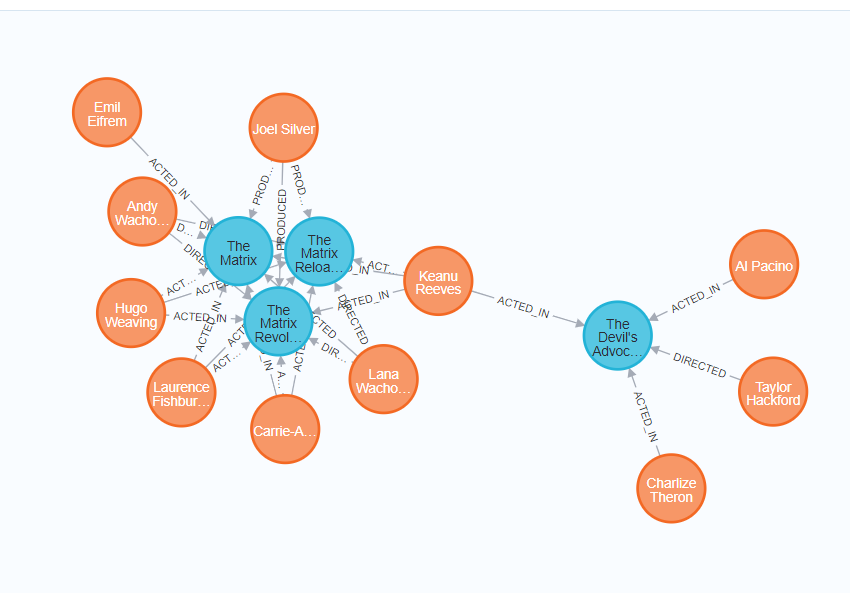
\includegraphics[scale=0.6]{Graficos/graph1.png}
    \caption{Gráfo de retorno según el tipo de nodo n como un pequeño segmento de toda la base de datos de películas}
    \label{fig:graph_1}
\end{figure}
Para nuestro segundo tipo de nodo tenemos como tag a película en el cual la Figura \ref{fig:tab_2} muestra un pequeño fragmento en forma de tabla de los nodos película y sus respectivos atributos:
\begin{itemize}
    \item Tagline: Frase representativa de dicha película.
    \item Title: Nombre de la película y el año en el que fue lanzada.
\end{itemize}
Después, es mostrado en forma de nodos de grafo las películas que ingresamos a nuestra base de datos en la Figura \ref{fig:graph_2}
\begin{figure}[H]
    \centering
    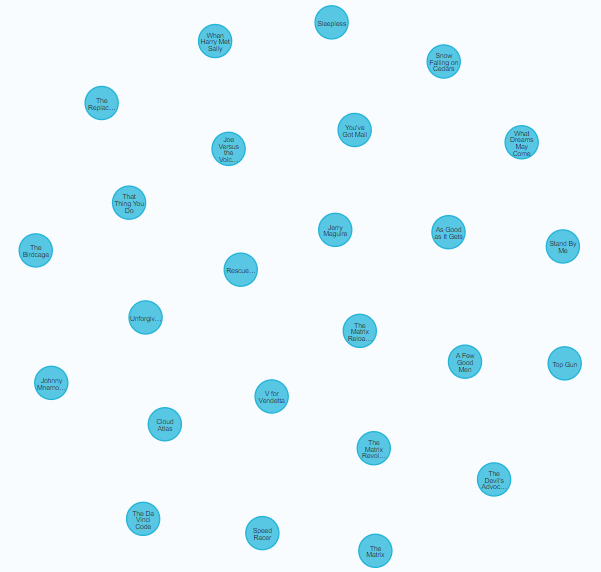
\includegraphics[scale=0.8]{Graficos/graph2.png}
    \caption{Grafo de nodos de películas sin relaciones ni conexiones.}
    \label{fig:graph_2}
\end{figure}
\begin{figure}[H]
    \centering
    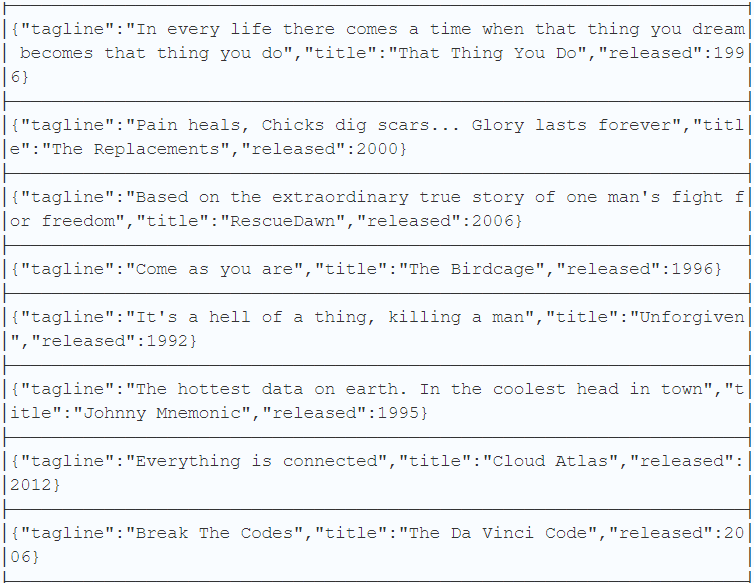
\includegraphics[scale=0.7]{Graficos/tabla2.png}
    \caption{Tabla de los nodos película de la base de datos}
    \label{fig:tab_2}
\end{figure}
Finalmente mostramos el tercer tipo de nodo de nuestra base de datos de películas el cual tiene de etiqueta person , el cual brinda los datos y atributos como muestra en la Figura \ref{fig:tab_3} que representan:
\begin{itemize}
    \item Actores.
    \item Escritores.
    \item Directores.
    \item Productores.
\end{itemize}
Y de manera general la Figura \ref{fig:tab_3} muestra como nodos sin conexiones ni relaciones los nodos person que existen en nuestra base de datos
\begin{figure}[H]
    \centering
    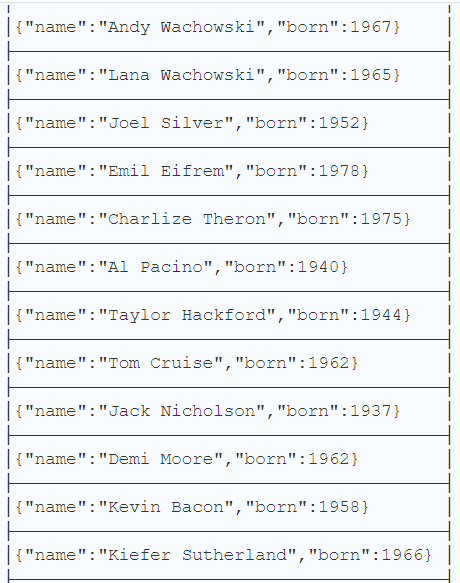
\includegraphics[scale=0.7]{Graficos/tab3.png}
    \caption{Tabla de los nodos person de la base de datos}
    \label{fig:tab_3}
\end{figure}
\begin{figure}[H]
    \centering
    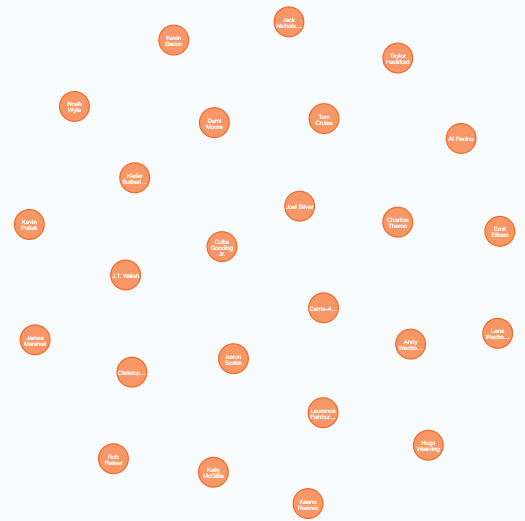
\includegraphics[scale=0.8]{Graficos/graph3.png}
    \caption{Nodos grafo con la etiqueta person de la base de datos de películas}
    \label{fig:graph_3}
\end{figure}
\subsection{Análisis de la base de datos}
\subsubsection{Consulta de los atributos de un nodo}
El objetivo es mostrar como se realizan para mostrar un nodo en concreto usando los comandos de consulta del lenguaje Cypher.\\
En la Figura \ref{fig:match_1} vemos en la sintaxis de escritura que se usa MATCH para referirse a un conjunto de nodos de un tipo representado por una variable el cual con LIMIT definimos la cantidad de nodos a mostrar.\\
En la Figura \ref{fig:match_2} notamos que ya explicitamente escogemos el nodo de una película buscandola por el título de esta para mostrar el título y el año en el que fue realizado dicha película.
\begin{itemize}
    \item Mostrar todos los nodos de un tipo en concreto , ya sea persona o película.
    \begin{figure}[H]
    \centering
    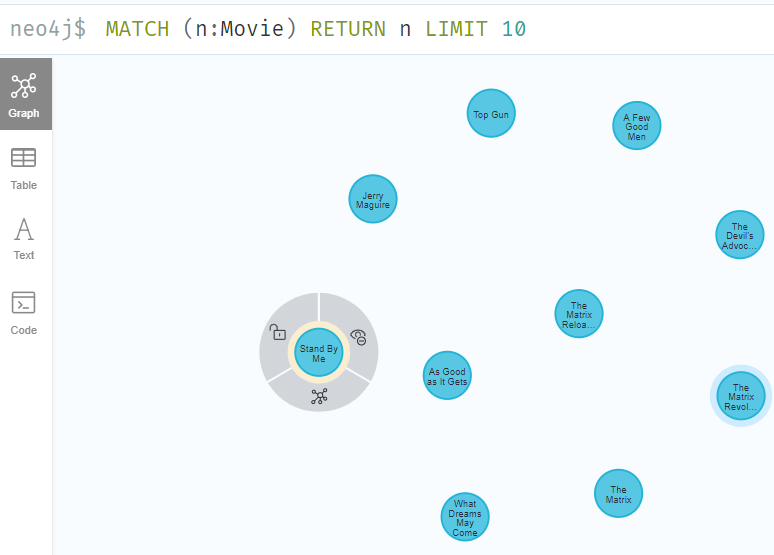
\includegraphics[scale=0.6]{Graficos/match1.png}
    \caption{Nodos película mostrados en grafo limitado a 10}
    \label{fig:match_1}
    \end{figure}
    \begin{figure}[H]
    \centering
    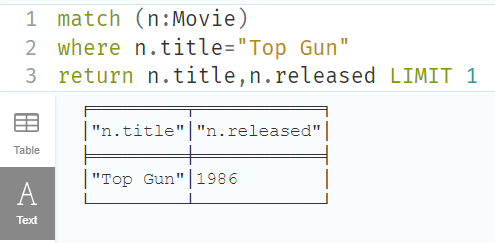
\includegraphics[scale=0.85]{Graficos/match2.png}
    \caption{Nodo película con titulo de Top Gun y su año en el que fue realizado}
    \label{fig:match_2}
    \end{figure}
    \item Mostrar un nodo y sus atributos en concreto
    En la Figura \ref{fig:att} vemos como un nodo película muestra sus relaciones con otros nodos en forma gráfica.
    \begin{figure}[H]
    \centering
    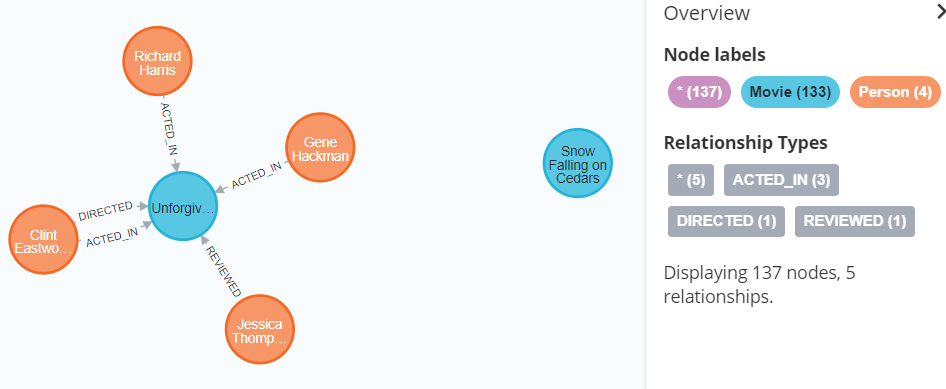
\includegraphics[scale=0.5]{Graficos/att.png}
    \caption{Nodo película Unforgiven con sus respectivas relaciones}
    \label{fig:att}
    \end{figure}
\end{itemize}
\subsubsection{Consulta encapsulada por diversos atributos}
En la Figura \ref{fig:peli} hacemos las búsquedas encapsuladas basadas en limitar el rango de búsqueda mediante un atributo en concreto.
\begin{figure}[H]
    \centering
    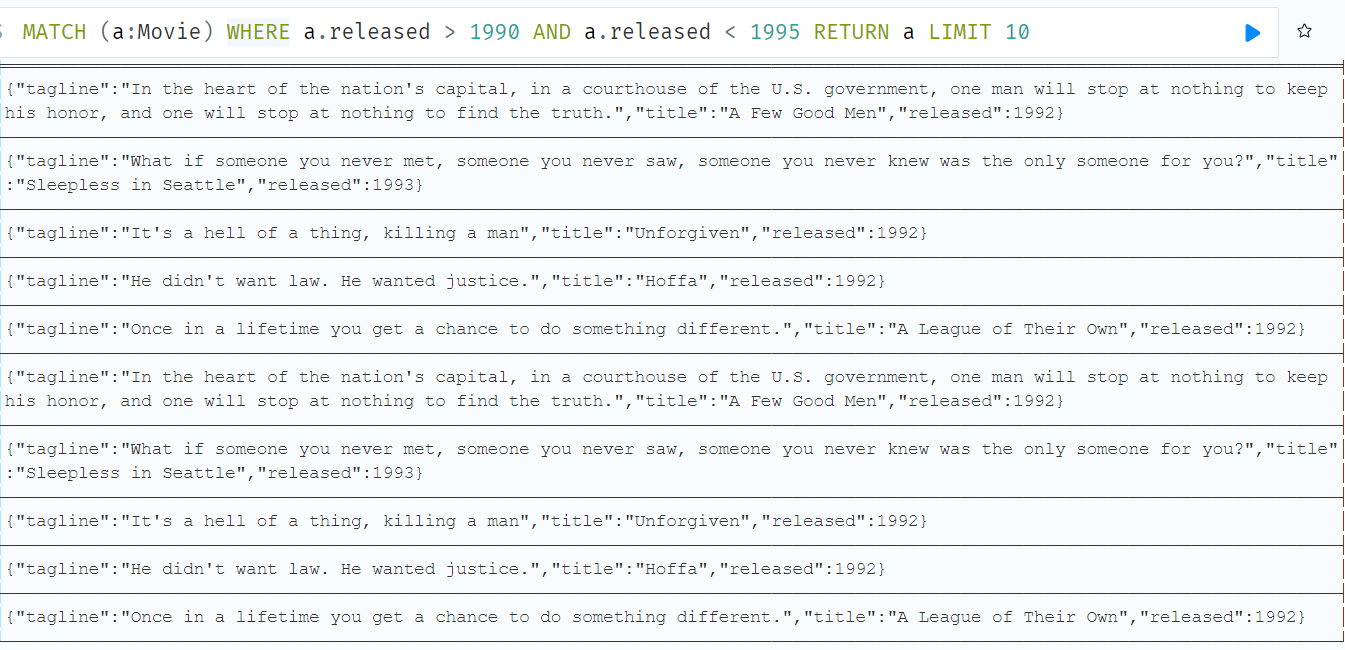
\includegraphics[scale=0.4]{Graficos/peli.png}
    \caption{Nodos película que se hayan realizado entre los años 1990 y 1995}
    \label{fig:peli}
\end{figure}
\subsubsection{Consultas complejas para evaluaciones complejas}
Para estas consultas tendremos un fin en concreto para hacer futuras relaciones.
\begin{itemize}
    \item Encontrar actores con los que cierto actor aún no haya trabajado, pero sus co-actores sí.
    En la Figura \ref{fig:coac} vemos como buscar a los coactores que no trabajaron con el actor Tom Cruise.
    \begin{figure}[H]
    \centering
    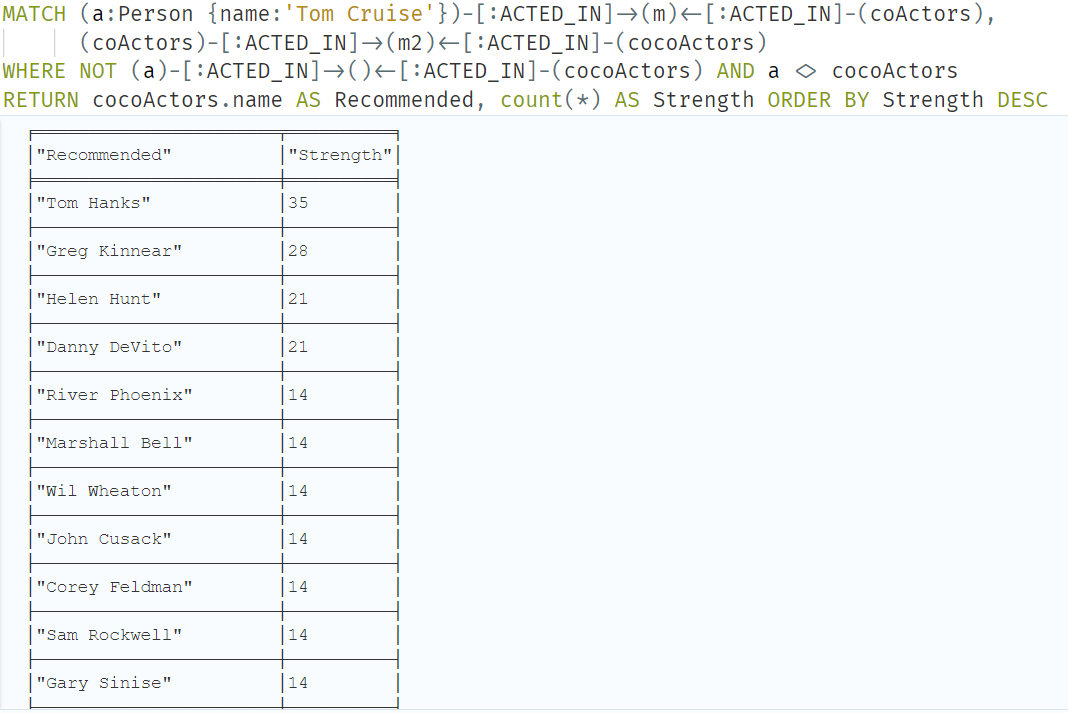
\includegraphics[scale=0.6]{Graficos/coactors.png}
    \caption{Tablero en orden descendente de la cantidad de coactores de actores principales}
    \label{fig:coac}
    \end{figure}
    \item Encontrar todas las personas que participaron en una película en concreto y que roles tuvieron en dicha película.
    En la Figura \ref{fig:inter} vemos como retornar todas las personas relacionadas a una película en concreto.
    \begin{figure}[H]
    \centering
    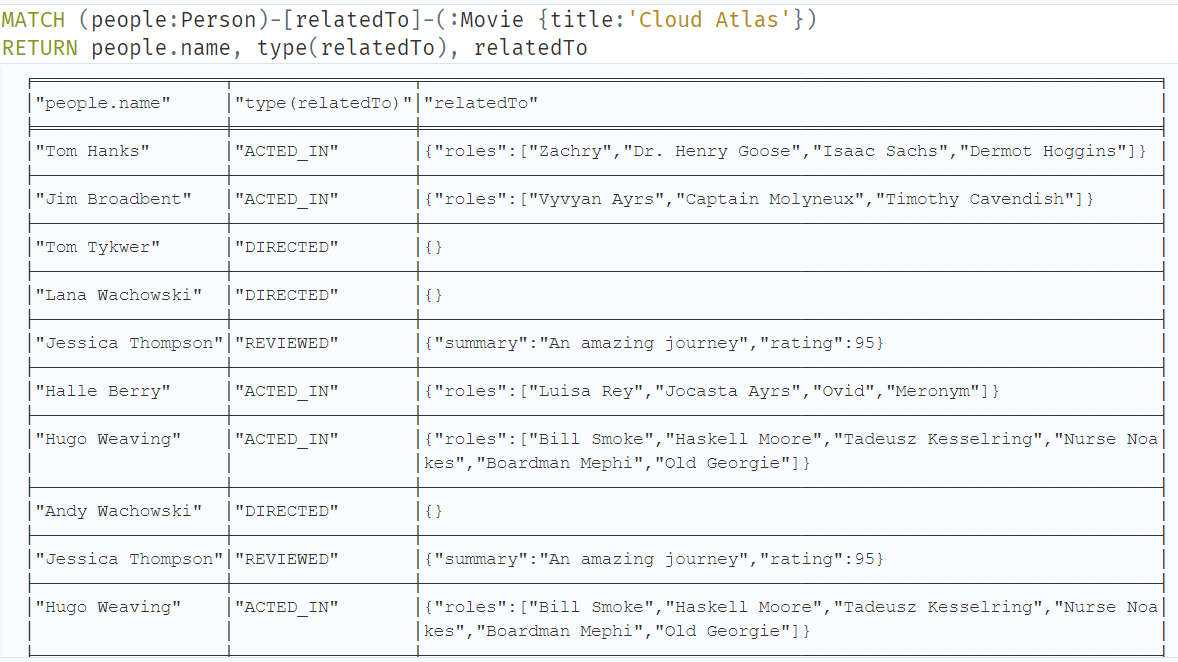
\includegraphics[scale=0.5]{Graficos/interact.png}
    \caption{Personas que interacturan en dicha película basada en las relaciones que tienen con esta.}
    \label{fig:inter}
    \end{figure}
\end{itemize}
\section{Base de datos de investigación universitaria en Neo4j}
Para los parámetros de evaluación de comparación no se tomará en cuenta el rendimiento ni la velocidad de ejecución de las consultas de dicho lenguaje, ya que, no se asegura saber que esten ejecutandose en las mismas condiciones.
Sin embargo, tomaremos en cuenta los siguientes aspectos:
\begin{itemize}
    \item Costo de la infrestructura.
    \item Velocidad de sintaxis (escritura y digitación de la misma).
    \item Comprensión del lenguaje.
    \item Facilidad de aprendizaje.
    \item Apoyo visual que sea atractivo, entendible y fácil de interpretar.
\end{itemize}
\subsection{Comparación SQL vs CYPHER Caso 1:}
La consulta de grafos escrita en Cypher es eficiente y simple. Podría decirse que puede ser formulado y realizado por trabajadores del conocimiento con menos experiencia que recibieron la formación previa y equipado con información tal como nodo y relación de nodo.
Además, la información visual que se muestra también es informativa y adecuada para diferentes niveles de espectadores, desde el conocimiento de  trabajadores a ejecutivos.\\
En la Figura \ref{fig:neo1} vemos la primera consulta en lenguaje cypher el cual consta de 1 linea de código cypher el cual realiza una unión entre resultados de búsqueda especificadas por las variables respectivas encontrando los artículos, autores y co-autores del proyecto de investigación buscado , muestra quienes interactuan de manera relacional con dicho proyecto de investigación.
Nos da la facilidad como desarrolladores o analistas de ver la cantidad de personas con sus respectivos roles y una imágen gráfica el cual representa la estructura de nodos y relaciones que involucran a dicho proyecto de investigación.\\
Una consulta más larga para responder a la misma pregunta en un relacional
La base de datos sería similar a la de la Figura \ref{fig:sql1}. La diferencia es clara. En una base de datos relacional, el requisito debe ser muy explícito por adelantado para que se traduzca correcta y cuidadosamente en consultas antes de decidir qué tablas unir en qué columnas y qué campos deben recuperarse. De hecho, requiere algunos nivel de experiencia técnica para ejecutarlo.
    \begin{figure}[H]
    \centering
    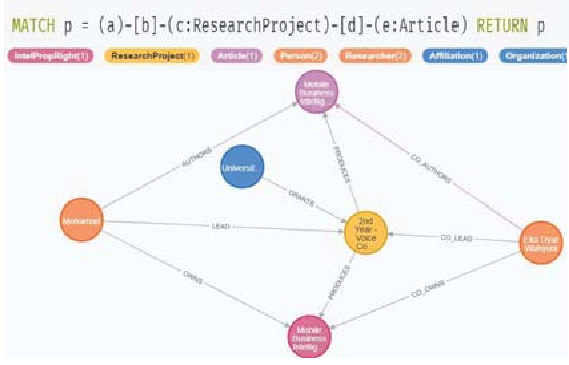
\includegraphics[scale=0.8]{Graficos/neo11.png}
    \caption{Caso 1: consulta Cypher}
    \label{fig:neo1}
    \end{figure}
    \begin{figure}[H]
    \centering
    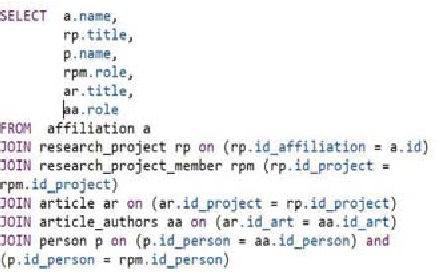
\includegraphics[scale=0.7]{Graficos/sql1.png}
    \caption{Caso 1 : Consulta SQL}
    \label{fig:sql1}
    \end{figure}+

\subsection{Comparación SQL vs CYPHER Caso 2:}
La consulta Cypher en la Figura \ref{fig:neo2} es abstracta y más natural
ya que las relaciones y los nodos subyacentes no son claramente
definido, pero solo se supone que existe. Sin embargo,los gráficos devueltos son informativos y brindan rápidamente información útil, que en una base de datos relacional es difícil de proporcionar.
Usando una base de datos relacional como se muestra en la Figura \ref{fig:sql2}, la consulta requiere pasos más largos, uniones y tiempo para ejecutarlo, especialmente cuando el tamaño de la base de datos es grande. Como la consulta anterior, es demasiado técnico y no fácilmente entendido por la gente en general y incluso trabajadores del conocimiento.

\begin{figure}[H]
    \centering
    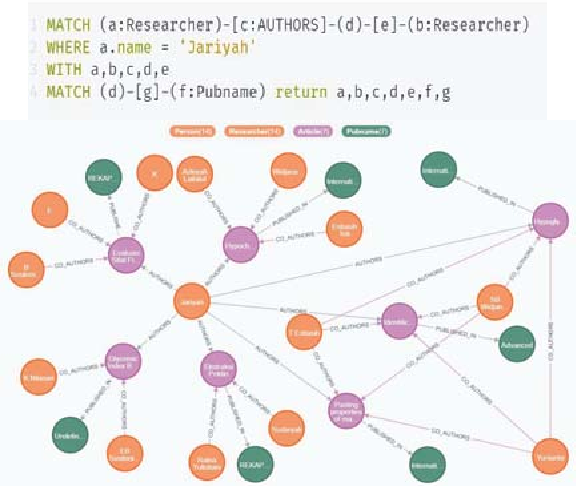
\includegraphics[scale=0.7]{Graficos/neo2.png}
    \caption{Caso 2 : Consulta Cypher}
    \label{fig:neo2}
    \end{figure}
\begin{figure}[H]
    \centering
    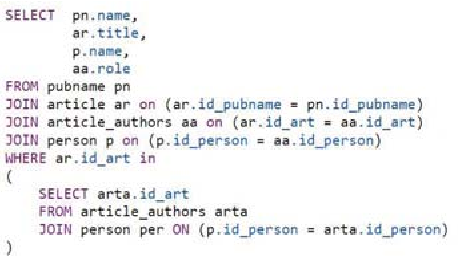
\includegraphics[scale=0.7]{Graficos/sql2.png}
    \caption{Caso 3 : Consulta SQL}
    \label{fig:sql2}
    \end{figure}
\subsection{Comparación SQL vs CYPHER Caso 3:}
Para el caso 3, la pregunta espera que exista(n) relación(es)
entre organizaciones de una forma u otra, ya sea directamente
o indirectamente. Una relación directa (a un enlace de distancia) sería algo así como Organización X HAS\_MOU\_WITH como Organización Y. Por otro lado, una conexión indirecta probablemente se manifestaría en algo como la Organización X EMPLEA a una Persona P que ESCRIBE un Artículo que es CO\_ESCRITO por una Persona P2 que TRABAJA para la Organización Y.
En este caso, hay cuatro relaciones entre Organización
X y Organización Y. La respuesta en CYPHER es tan natural
como puede ser, como se muestra en la Figura \ref{fig:neo3}.
Como se demostró en el caso 1, caso 2 y caso 3, el gráfico
la base de datos y la consulta hacen el trabajo de responder consultas
de manera eficiente en comparación con la base de datos relacional. Estos simples experimentos están en línea con estudios previos que compararon
base de datos de gráficos (neo4j) y otros sistemas de bases de datos.
Los resultados también revelan que las consultas gráficas formuladas
están muy cerca de los lenguajes naturales indicados en las consultas de perspectivas múltiples. Para directores o líderes universitarios que
a menudo se encuentran en medio de reuniones en las que se les solicita
para proporcionar información aleatoria y ad-hoc sobre su
universidades, las capacidades de las consultas gráficas sin duda serán
beneficioso.
Además de las funciones de informes y análisis compatibles
por consultas y bases de datos relacionales, que la mayoría de los ejecutivos
Los sistemas de información (EIS) que tienen actualmente, las organizaciones pueden necesitar desarrollar capacidades gráficas y analíticas respaldadas
por bases de datos gráficas y consultas.
Estudios previos por capacidades de chatbot agregadas
a la EIS existente para que los ejecutivos puedan ver y obtener
información sobre sus universidades ordenando a través de
voces y textos. Los problemas con esos sistemas son que no se sabe más allá del conocimiento específico incrustado en ellos.
Los comandos son limitados porque ellos y sus consultas SQL asociadas deben estar predefinidos primero. Entonces, esos sistemas tienen solicitudes de información aleatorias y ad hoc no atendidas.
La base de datos de gráficos y las consultas tienen grandes posibilidades de
superar ese problema. Pueden entender y producir los resultados de manera intuitiva a pesar de las preguntas a ciegas, que parecen difíciles de
comprender y parecer sin sentido, como se muestra en el Caso 1 y
Caso 2. El nodo-relación-nodo posiblemente se convertirá en el
clave en la interpretación de solicitudes aleatorias de información siempre que
podemos mapear cosas a nodos en la base de datos. De hecho, la implementación seguirá siendo un desafío, especialmente cuando se integran datos de diferentes bases de datos, a menudo sistemas heredados, donde la documentación está menos disponible o no existe.
\begin{figure}[H]
    \centering
    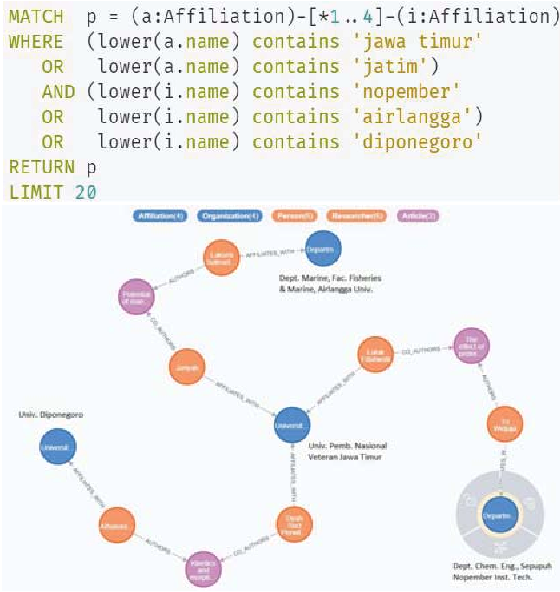
\includegraphics[scale=0.8]{Graficos/neo33.png}
    \caption{Caso 3 : Consulta Cypher}
    \label{fig:neo3}
    \end{figure}
\subsection{Ventajas que propone el Neo4j con la base de datos en lenguaje Cypher}
Al basarnos en un sistema en concreto, trabajando con una base de datos de investigadores para el respaldo de la información de los estudiantes universitarios, se detectó las siguientes ventajas:
\begin{itemize}
    \item La base de datos de gráficos de investigación presentada en este estudio tiene demostrado responder de manera eficiente a las consultas en comparación con la base de datos relacional.
    \item La base de datos de gráficos de investigación presentada en este estudio proporcionan visualmente atractivos discernimiento.
    \item La sintaxis del lengua Cypher se asemeja al lenguaje natural para la correcta interpretación de una persona con un conocimiento promedio de dicha disciplina, apoyado de un material visual que respalda dicha sintaxis.
    \item Sql es destacado por ser un lenguaje usado netamente por programadores de mucha experiencia, los cuales tienen mucho tiempo estudiando no solo el entorno de bases de datos sino también el lenguaje de SQL, como realizar transacciones y consultas correspondientes, sin embargo, se apoyan de herramientas como la ingeniería reversa para plasmar sus arquitecturas en tablas organizacionales las cuales muestran de manera robótica los nodos y relaciones.
    \item Las consultas SQL extensas no solo requieren más tiempo para ejecutarse, sino que también es más probable que incluyan errores de codificación humana debido a su complejidad. Además, las consultas más breves aumentan la facilidad de comprensión y mantenimiento en todo su equipo de desarrolladores.
    \item Cypher está diseñado para que los desarrolladores, los profesionales de bases de datos y las partes interesadas del negocio lo lean y entiendan fácilmente. Es fácil de usar porque coincide con la forma en que describimos intuitivamente los gráficos mediante diagramas.
    \item La noción básica de Cypher es que le permite pedirle a la base de datos que busque datos que coincidan con un patrón específico. Coloquialmente, podríamos pedirle a la base de datos que “encuentre cosas como esta”, y la forma en que describimos cómo se ven “cosas como esta” es dibujándolas usando arte ASCII .
    \item Un lenguaje de consulta representa su modelo de cerca. Es por eso que SQL se trata de tablas y JOIN, mientras que Cypher se trata de relaciones entre entidades. Tanto como el modelo gráfico es más natural para trabajar, también lo es Cypher, ya que toma prestado de la representación pictórica de círculos conectados con flechas que cualquier interesado (ya sea técnico o no técnico) puede entender.
    \item En una base de datos relacional, el proceso de modelado de datos se abstrae hasta ahora de las consultas SQL reales del día a día que existe una gran disparidad entre el análisis y la implementación. En otras palabras, el proceso de construcción de un modelo de base de datos relacional no es adecuado para hacer (y responder) preguntas de manera eficiente desde ese mismo modelo.
    Los modelos de bases de datos de gráficos, por otro lado, no solo comunican cómo se relacionan sus datos, sino que también lo ayudan a comunicar claramente los tipos de preguntas que desea hacer sobre su modelo de datos. Los modelos gráficos y las consultas gráficas son solo dos caras de la misma moneda.

\end{itemize}
\chapter{Resultados y/o Discusión}
\hrule \bigskip \vspace*{1cm}
%------------------------------------------------------------------------
\subsection{Neo4j como la mejor opción de BD}
Después de haber reproducido todas las técnicas correspondientes, notamos que Neo4j es mejor que SQL tanto en sintaxis como en aprendizaje para programadores que recien se adentran a esta rama,\\
Neo4j no solo te brinda una sintaxis mas entendible y reducida, sino también te brinda una gráfica que te permite entender mejor la consulta y relaciones de tu base de datos sin estar realizando comandos como select, join y demás para mostrar lo que deseas.\\
Los colores interactivos que brinda su gráfica hace el trabajo de análisis y comprensión menos tediosa.\\
En la comparación vemos que \ref{fig:neo2} y \ref{fig:sql2} presentan muchas diferencias las cuales ya analizamos con anterioridad.
\begin{figure}[H]
    \centering
    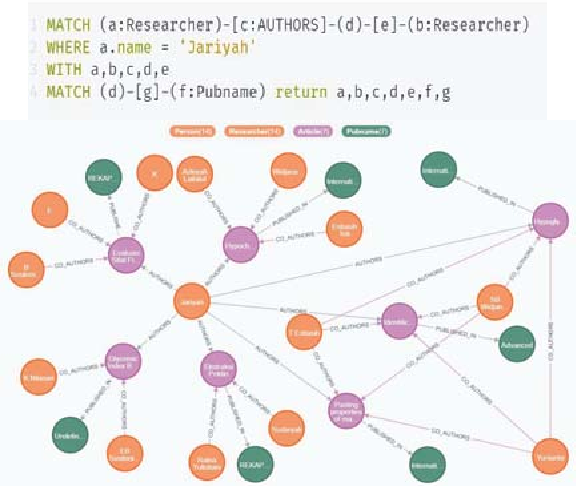
\includegraphics[scale=0.7]{Graficos/neo2.png}
    \caption{Caso 2 : Consulta Cypher}
    \label{fig:neo2}
    \end{figure}
\begin{figure}[H]
    \centering
    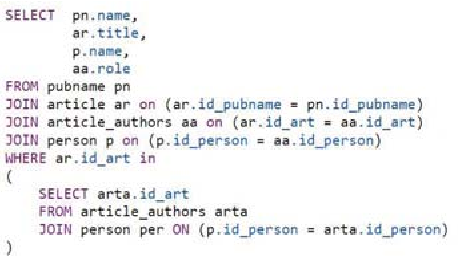
\includegraphics[scale=0.7]{Graficos/sql2.png}
    \caption{Caso 3 : Consulta SQL}
    \label{fig:sql2}
    \end{figure}

\subsection{Neo4j como la mejor opción para analístas}
La herramienta propuesta no solo brinda una gráfica iteractiva sino que además muestra las relaciones que posiblemente puedan llevarte a un objetivo que estes buscando.\\
Muestra toda la información correspondiente de cada nodo con su respectiva relación de la cual quisieras información y los posibles nodos que se vieran involucrados.
\begin{figure}[H]
    \centering
    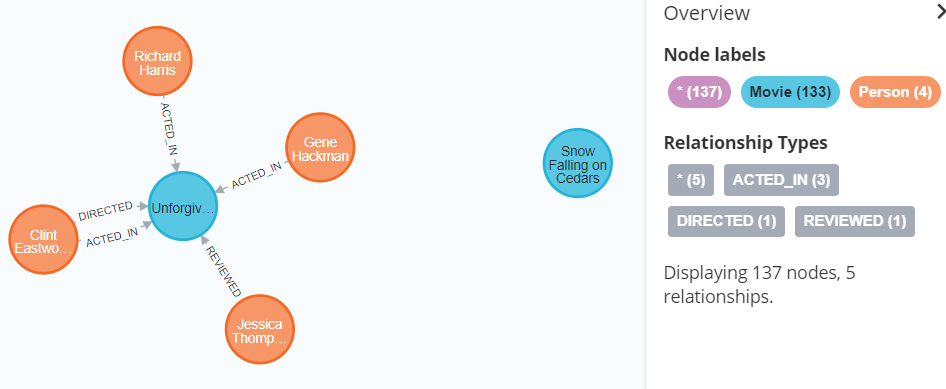
\includegraphics[scale=0.5]{Graficos/att.png}
    \caption{Nodo película Unforgiven con sus respectivas relaciones}
    \label{fig:att}
    \end{figure}
\subsection{Concytec como Información Valiosa}
En la técnica 2 pudimos evaluar como usan google schoolar como base de datos de investigadores para el mismo propósito de este papper, hacer que los universitarios tengan el mayor respaldo y asesoramiento posible de la manera mas accesible que puedan encontrar.\\
Concytec asi como google schoolar, brindan cierta información valiosa para un universitario el cual le permitirá elegir mejor a su asesor de acuerdo a lo que requieran. La segunda técnica mostró que es una necesidad realizar este tipo de propuestas para hacer que grupos de investigación como el que tiene concytec puedan ayudar a los demás.
\begin{figure}[H]
    \centering
    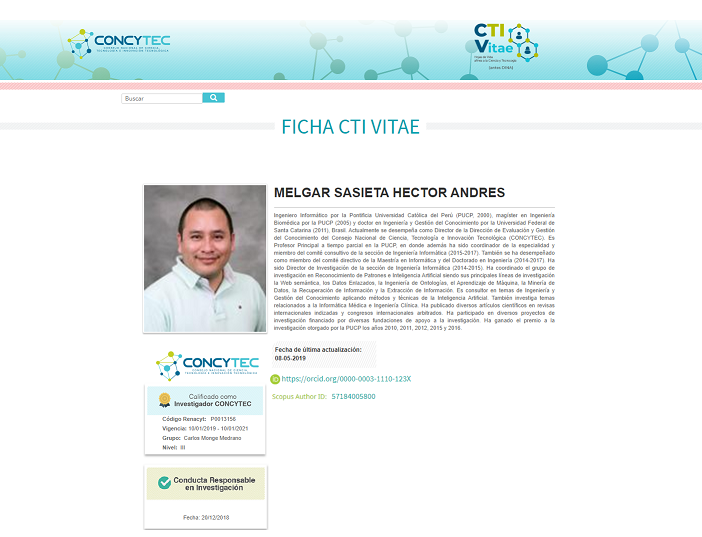
\includegraphics[scale=0.6]{Graficos/concytec.png}
    \caption{CV de profesor en la página de concytec}
    \label{fig:att}
    \end{figure}
\chapter{Conclusiones y trabajo futuro}
\hrule \bigskip \vspace*{1cm}
%------------------------------------------------------------------------

\section{Conclusiones}

Al desarrollar este trabajo de investigación y apoyarnos de dos técnicas tanto informativas e introductorias como comparativas para nuestro análisis y resultado obtenido, notamos que, fue una elección correcta el elegir a Cypher como lenguaje de programación y a Neo4j como herramienta para nuestra investigación.\\
De entre tantas fuentes de información es importante elegir una de las más accesibles para el investigador, en este caso, Concytec. Al evaluar dichas fuentes de información similares a esta, vimos que , el avance de investigación para el reforzamiento de asesorias y respaldo para los investigadores es impresindible para lograr una mejor y más asertiva búsqueda con las herramientas correctas,


\section{Trabajos futuros}
Se plantea como trabajo futuro realizar una aplicación para la página de concytec el cual recopile la información de los CV de los investigadores y así hacer el llenado de nuestra base de datos orientada a grafos de manera automática, el cual facilitaría la recopilación de datos y podría ampliar nuestro avance de investigación planteado en este artículo.




\printglossaries
%\myappendix{Apendice}
\begin{singlespace}
\bibliographystyle{apalike}%plain
\mybibliography{biblio}
\end{singlespace}





\end{document}%%%%%%%%--------------------------------------------------------
